\section{eo\-Real\-Init\-Bounded$<$ EOT $>$ Class Template Reference}
\label{classeo_real_init_bounded}\index{eoRealInitBounded@{eoRealInitBounded}}
Simple initialization for any EOT that derives from std::vector$<$double$>$ uniformly in some bounds.  


{\tt \#include $<$eo\-Real\-Init\-Bounded.h$>$}

Inheritance diagram for eo\-Real\-Init\-Bounded$<$ EOT $>$::\begin{figure}[H]
\begin{center}
\leavevmode
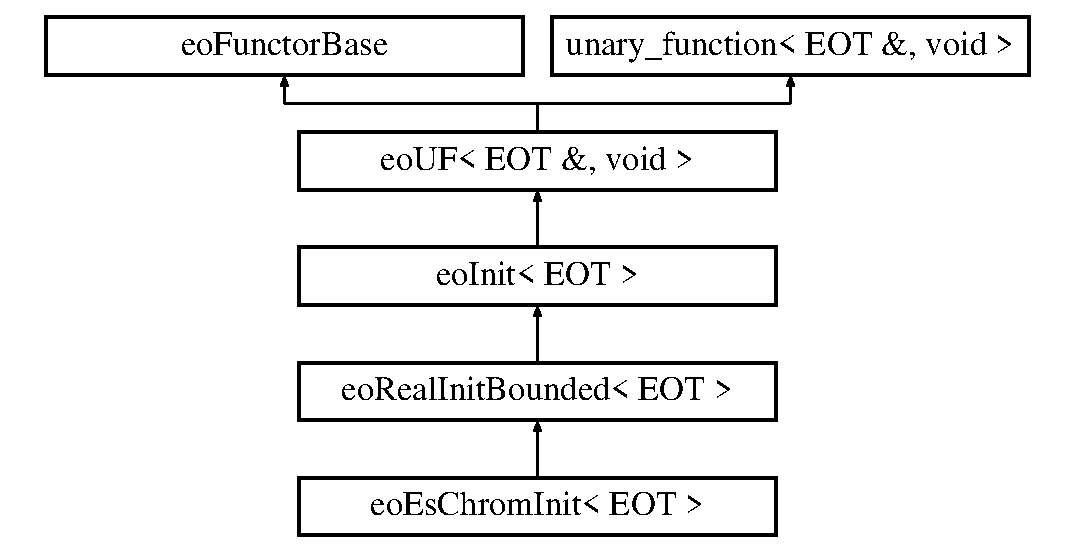
\includegraphics[height=5cm]{classeo_real_init_bounded}
\end{center}
\end{figure}
\subsection*{Public Member Functions}
\begin{CompactItemize}
\item 
{\bf eo\-Real\-Init\-Bounded} ({\bf eo\-Real\-Vector\-Bounds} \&\_\-bounds)\label{classeo_real_init_bounded_a0}

\begin{CompactList}\small\item\em Ctor - from {\bf eo\-Real\-Vector\-Bounds}{\rm (p.\,\pageref{classeo_real_vector_bounds})}. \item\end{CompactList}\item 
virtual void {\bf operator()} ({\bf EOT} \&\_\-eo)\label{classeo_real_init_bounded_a1}

\begin{CompactList}\small\item\em simply passes the argument to the uniform method of the bounds \item\end{CompactList}\item 
virtual {\bf eo\-Real\-Vector\-Bounds} \& {\bf the\-Bounds} ()\label{classeo_real_init_bounded_a2}

\begin{CompactList}\small\item\em accessor to the bounds \item\end{CompactList}\item 
virtual unsigned {\bf size} ()\label{classeo_real_init_bounded_a3}

\end{CompactItemize}
\subsection*{Private Attributes}
\begin{CompactItemize}
\item 
{\bf eo\-Real\-Vector\-Bounds} \& {\bf bounds}\label{classeo_real_init_bounded_r0}

\end{CompactItemize}


\subsection{Detailed Description}
\subsubsection*{template$<$class EOT$>$ class eo\-Real\-Init\-Bounded$<$ EOT $>$}

Simple initialization for any EOT that derives from std::vector$<$double$>$ uniformly in some bounds. 



Definition at line 40 of file eo\-Real\-Init\-Bounded.h.

The documentation for this class was generated from the following file:\begin{CompactItemize}
\item 
eo\-Real\-Init\-Bounded.h\end{CompactItemize}
